\documentclass[11pt,letterpaper]{article}
\usepackage[T1]{fontenc}
\usepackage[utf8]{inputenc}
\usepackage{amsmath}
\usepackage{newtxtext,newtxmath}
\usepackage[left=1.1in,right=1.1in,top=0.95in,bottom=0.9in]{geometry}
\usepackage{graphicx}
\usepackage{booktabs,tabularx,array}
\usepackage{enumitem}
\usepackage{microtype}
\usepackage{titlesec}
\usepackage[labelfont=bf,labelsep=period,font=small,justification=justified]{caption}
\usepackage{cite}
\usepackage{url}
\usepackage[hidelinks]{hyperref}

\captionsetup[figure]{name=Fig.,skip=5pt}
\captionsetup[table]{justification=centering,skip=4pt}
\titleformat{\section}{\fontsize{12}{14}\selectfont\bfseries}{\thesection}{0.5em}{}
\titleformat{\subsection}{\fontsize{11}{13}\selectfont\bfseries\itshape}{\thesubsection}{0.5em}{}
\titlespacing*{\section}{0pt}{13pt}{4pt}
\titlespacing*{\subsection}{0pt}{9pt}{3pt}
\setlength{\parindent}{0pt}
\setlength{\parskip}{5pt plus 1pt}
\setlist{itemsep=2pt,topsep=2pt,parsep=0pt}
\newcolumntype{Y}{>{\raggedright\arraybackslash}X}
\renewcommand{\arraystretch}{1.12}
\urlstyle{same}
\setcounter{secnumdepth}{0}
\setlength{\emergencystretch}{2em}

\begin{document}

\begin{center}
{\fontsize{17}{21}\selectfont\bfseries Beyond Accuracy: Evaluating Phishing Intent Discrimination in LLM-Generated Emails Using Matched Benign Controls\par}
\vspace{12pt}
{\fontsize{12}{14}\selectfont \makebox[0.82\linewidth]{Devarsh Ganatra\hfill Alok Singh\hfill Arrsh Tripathi}\par}
\end{center}
\vspace{6pt}
\begin{list}{}{\leftmargin=0.35in\rightmargin=0.35in}\small\item[]
\textbf{Abstract.} Phishing detectors built on fine-tuned Transformer encoders score close to perfectly on public email corpora, yet they degrade sharply on phishing written by large language models (LLMs). Earlier reports of this collapse compared two unrelated datasets, so they could not say whether detectors fail because the text is machine-written, because its register differs, or because the detector never learned what phishing is. We built a scenario-matched evaluation set that holds surface cues constant while varying intent. For each of ten attack scenarios and three generators (allam-2-7b, qwen3.8-27b, gpt-oss-20b), we produced a phishing email, a legitimate twin that keeps the same surface cues (deadline, link, authority figure), a plain legitimate email, and register rewrites of the first two, giving 1,446 emails. Seven DistilBERT variants, with and without handcrafted perplexity, grammar, length, urgency, fear and authority features, were each trained with five seeds on 17,566 emails, alongside a TF-IDF logistic-regression baseline trained on the same split. On the conventional test split every model reached F1 $\approx$ 0.987 and ROC-AUC $\approx$ 0.999. On the matched pairs, DistilBERT separated phishing from its legitimate twin with an AUC of only 0.62 (95\% cluster-bootstrap CI 0.57--0.68), against 0.78 for plain legitimate mail, and it flagged 37\% of the legitimate twins. No handcrafted feature closed this gap. Perplexity and grammar-error rate distinguished the conventional corpus from LLM-generated text (AUC 0.89 and 0.96) but not phishing from its twin (0.52 and 0.57). The lexical baseline separated intent better (AUC 0.75) but still raised false alarms on 41\% of the twins. Both model families missed nearly all document-sharing lures. A blinded two-annotator audit confirmed most twin labels ($\kappa$ = 0.55), and excluding disputed twins left the result unchanged. RoBERTa-base (AUC 0.68) and an external benchmark, E-PhishLLM, reproduced the pattern. High accuracy on the conventional corpus did not predict intent discrimination on LLM-generated mail, and evaluation sets for this task should contain matched benign controls.

\textbf{Keywords:} phishing detection; large language models; distribution shift; shortcut learning; contrast sets; DistilBERT; feature fusion; email security
\end{list}
\vspace{4pt}

\section{1. Introduction}

Phishing attacks frequently exploit persuasive communication. An attacker borrows the voice of an authority, adds a deadline, and asks for one small action: a click, a login, a payment \cite{ferreira2015}. Automated defences followed the attackers from structural and header features \cite{fette2007} to natural-language features \cite{verma2012}, and then to Transformer encoders \cite{vaswani2017,devlin2019,sanh2019} fine-tuned on labelled mail \cite{lee2020,jamal2023}. On public benchmarks these encoders now report accuracy approaching 99\%, although such results do not establish robustness under distribution shift.

LLMs complicate that picture. Hazell showed that GPT-4 can write tailored spear-phishing for hundreds of targets at a fraction of a cent each \cite{hazell2023}. In human-subject studies, GPT-4-written phishing drew more clicks than generic controls \cite{heiding2024}, and a fully automated LLM pipeline matched human experts \cite{heiding2024b}. In a field study at a large university, LLM-written lateral phishing was about as effective as messages written by professional communications staff \cite{bethany2025}. On the defensive side, SpearBot reported that BERT, RoBERTa and GPT-2 detectors trained on legacy corpora caught only a few percent of LLM-refined spear-phishing \cite{qi2025}, and E-PhishGen showed that detectors near ceiling on established datasets lose much of their accuracy on a newer, LLM-generated benchmark \cite{pajola2025}.

These studies document performance degradation, but their designs do not fully isolate its causes. In each comparison the training and test sets differ at once in source, period, topic, sender, class balance, generator and writing style, so it is hard to say which of these differences is responsible. A drop in recall is consistent with at least three different stories. The detector may not recognise machine-written text; it may rely on the register of the training corpus, so that polished corporate prose reads as safe; or it may never have learned phishing intent at all, only the vocabulary that happened to accompany phishing in its training data. These explanations call for different fixes, and the usual evaluation cannot tell them apart. We therefore ask a narrower question: does a fine-tuned detector distinguish a malicious request from a legitimate message that carries the same surface cues? The same ambiguity affects work that adds handcrafted signals to an encoder: when psychological trait scores \cite{shahriar2022} or likelihood statistics improve recall on a shifted test set, it is unclear whether they help the model find phishing or simply mark text that looks unfamiliar.

Security research and machine learning research have both warned about this kind of uncontrolled comparison. Arp et al. list spurious correlations and inappropriate baselines among the most common pitfalls in security ML \cite{arp2022}, and work on distribution shift shows that in-distribution accuracy is a weak guide to behaviour on new data \cite{koh2021}. The standard remedy in NLP is to probe a model with minimally different inputs whose labels differ. Contrast sets \cite{gardner2020} and counterfactually revised examples \cite{kaushik2020} expose models that solve a benchmark through shortcuts \cite{geirhos2020} rather than through the property the benchmark was meant to measure.

We apply that remedy to phishing detection. For each attack scenario we generate a phishing email (P) and a legitimate twin ($B_{\mathrm{hard}}$) that keeps the same sender role, topic and cues (a deadline, a link, an appeal to authority) but has benign intent. A plain legitimate email ($B_{\mathrm{easy}}$) gives a reference point without those cues. We then rewrite P and $B_{\mathrm{hard}}$ into a different register \cite{biber1988variation} while preserving facts and intent ($P_{\mathrm{R}}$, $B_{\mathrm{hard,R}}$). A detector sensitive to malicious intent should distinguish P from $B_{\mathrm{hard}}$. A detector driven by register should change its score at least as much when an email is rewritten as when its intent is flipped. We use this design to answer five research questions.

\begin{itemize}
\item \textbf{RQ1 (degradation).} How large is the gap between performance on the conventional test split and on matched LLM-written pairs, and how stable is it across training seeds and generators?
\item \textbf{RQ2 (intent).} Can fine-tuned detectors separate a phishing email from a legitimate email that carries the same surface cues?
\item \textbf{RQ3 (register).} Does an intent-preserving change of register move detector scores more than a change of intent does?
\item \textbf{RQ4 (features).} What do the handcrafted behavioural (perplexity, grammar-error rate, length) and psychological (urgency, fear, authority) features measure, and does adding them to DistilBERT improve intent recognition?
\item \textbf{RQ5 (lexical baseline).} How does a TF-IDF logistic-regression model trained on the same data behave on the matched pairs, and how much of its apparent robustness is real?
\end{itemize}

The paper makes four contributions.

\begin{enumerate}
\item A scenario-matched evaluation set of 1,446 LLM-written emails over three generators, ten scenarios and five conditions, with a log of every generation attempt and its outcome, including refusals, and a blinded two-annotator audit of the benign twins.
\item A single-feature ablation of DistilBERT with five seeds per variant (35 models), a RoBERTa-base comparison and an external benchmark, analysed with paired tests on per-email predictions.
\item Evidence that every DistilBERT variant separates phishing from its legitimate twin only slightly better than chance despite near-perfect in-distribution scores, together with a measurement of what the added features encode.
\item Evidence that a lexical baseline separates intent better than the encoders, that this advantage survives the removal of corpus-provenance tokens, and that both model families share the same blind spots on workplace lures.
\end{enumerate}

Section 2 reviews related work. Section 3 describes the data, the matched-pair design, the models and the pre-specified hypotheses, and Section 4 summarises the implementation. Section 5 reports results, Section 6 answers the research questions and discusses implications, Section 7 sets out limitations, and Section 8 concludes.

\section{2. Related Work}

\subsection{2.1 LLM-enabled phishing}

The offensive literature is now consistent. LLMs can collect background on a target and write convincing messages at low reported generation cost \cite{hazell2023}. Heiding et al. found that GPT-4-written phishing drew more clicks than generic controls, though fewer than emails designed with a human persuasion framework \cite{heiding2024}, and a later fully automated pipeline matched human experts at 54\% click-through against 12\% for controls \cite{heiding2024b}. Bethany et al. ran an eleven-month study with about 9,000 university staff and found LLM-written lateral phishing roughly as effective as emails written by communications professionals \cite{bethany2025}. SpearBot pairs a generator with LLM critics and refines each email until the critics stop flagging it; detectors trained on legacy corpora then catch almost none of the output \cite{qi2025}. E-PhishGen generated a balanced, multilingual benchmark of 16,616 emails and found that detectors near ceiling on older datasets lose substantial accuracy on it \cite{pajola2025}. Our work starts where these studies stop: we ask what the degraded detectors are actually responding to.

\subsection{2.2 Feature-based, psychological and Transformer detectors}

Early detectors used link, domain and HTML features \cite{fette2007}, and later work added linguistic analysis \cite{verma2012}. Ferreira and Lenzini traced effective phishing to persuasion principles such as authority and urgency \cite{ferreira2015}, following Cialdini's account of influence \cite{cialdini2006influence}. Shahriar et al. are the closest prior work on psychological features: they trained trait scorers for urgency, fear and enticement and concatenated the scores with BERT and SBERT representations, improving F1 over earlier systems \cite{shahriar2022}. They used GPT-2 output only to augment training data. Their trait scores are learned by trained models; our psychological features are fixed keyword and entity counts. The present study therefore does not propose a new psychological-feature fusion method; it tests simple cue counts against matched benign twins rather than on a conventional split.

Transformer encoders \cite{vaswani2017,devlin2019} and their compressed and improved forms \cite{sanh2019,liu2019,he2021} are widely used as backbones for phishing detection. CATBERT adds header context to a compressed BERT \cite{lee2020}, and Jamal and Wimmer fine-tune BERT-family models for phishing and spam \cite{jamal2023}. SecureNet compares DeBERTa with GPT-4 and Gemini and finds the fine-tuned encoder slightly ahead on recall \cite{mahendru2024}. A second line of work uses LLMs as detectors: ChatSpamDetector prompts GPT-4 with the raw email and reports high accuracy with written rationales \cite{koide2025}, and PiMRef checks the sender's claimed identity against a knowledge base instead of judging style \cite{liu2025}. Kulal et al. evaluate conventional, LLM-generated and character-level adversarial phishing, but their LLM set contains 88 phishing emails and no benign LLM text \cite{kulal2025}.

\subsection{2.3 Dataset artefacts and corpus provenance}

Public phishing corpora are assembled from sources of different origin and age. Legitimate mail often comes from the Enron collection \cite{klimt2004}, and phishing from older spam and phishing archives; the public Kaggle collection used here is one such merge \cite{subaiey2024}, and recent curation efforts document the mix \cite{champa2024,mendes2025}. Verma et al. warned that phishing datasets carry quality problems that inflate reported accuracy \cite{verma2019}. Most directly, Bhuiyan and Bhuiyan show that TF-IDF classifiers can identify which of six classical corpora an email came from with 97--98\% accuracy, so part of what they learn is provenance rather than phishing \cite{bhuiyan2026}. Similar spatial and temporal biases have been documented in malware detection \cite{pendlebury2019} and, earlier, in intrusion detection \cite{sommer2010}.

\subsection{2.4 Shortcut learning and contrast evaluation}

Models often solve a benchmark with a cue that is correlated with the label in the training data but not with the property the label describes \cite{geirhos2020}. Natural language inference models exploit annotation artefacts in hypotheses \cite{gururangan2018} and lexical overlap heuristics \cite{mccoy2019}, and argument comprehension models exploit cue words \cite{niven2019}. Gardner et al. proposed contrast sets, small manual perturbations of test items that flip the gold label, to probe a model's local decision boundary; models lost up to 25 points on them \cite{gardner2020}. Kaushik et al. showed that counterfactually revised examples expose and reduce reliance on spurious features \cite{kaushik2020}, and CheckList organises such behavioural tests systematically \cite{ribeiro2020}. We apply contrast-set principles to phishing detection, where the natural minimal edit is a legitimate email that keeps every cue of the phishing email but drops its malicious request.

\subsection{2.5 Machine-generated text signals and register}

Token-likelihood statistics can separate generated from human text \cite{gehrmann2019,ippolito2020,mitchell2023}, and perplexity under a fixed model such as GPT-2 \cite{radford2019language} is the simplest of them. These signals are fragile. Paraphrasing defeats several detector families \cite{sadasivan2023}, and a dedicated paraphraser reduced DetectGPT's detection rate from 70.3\% to 4.6\% at a 1\% false-positive rate \cite{krishna2023}. Liang et al. found that GPT detectors flag over half of essays by non-native English writers as machine-written, because plain, predictable wording lowers perplexity \cite{liang2023}. Perplexity therefore tracks writing style as much as authorship. We use the term register in the sense of Biber and Conrad: language variation tied to the situation and purpose of communication, such as a terse internal note versus a courteous customer-service message \cite{biber1988variation,biber2009register}.

\subsection{2.6 Positioning}

Table 1 compares the present study with the closest work. It compares study designs rather than performance; none of these systems was evaluated on our data.

\begin{table}[!htbp]
\centering
\footnotesize
\caption{Positioning against the closest studies.}
\begin{tabularx}{\linewidth}{YYYYYY}
\toprule
\textbf{Study} & \textbf{Detectors} & \textbf{LLM-written test data} & \textbf{Benign LLM controls} & \textbf{Intent-matched pairs} & \textbf{Variance and paired tests} \\
\midrule
Shahriar et al. \cite{shahriar2022} & BERT/SBERT + trait scores & No (GPT-2 used for augmentation) & No & No & Not reported \\
SpearBot \cite{qi2025} & BERT, RoBERTa, GPT-2, classical ML & Yes, adversarially refined & No & No & Not reported \\
E-PhishGen \cite{pajola2025} & DistilBERT, TF-IDF-based models & Yes, 16,616 emails & Yes & No & Repeated trials \\
Kulal et al. \cite{kulal2025} & Classical ML with embeddings & Yes, 88 emails & No & No & Not reported \\
Bhuiyan and Bhuiyan \cite{bhuiyan2026} & TF-IDF LR, linear SVC & No & Not applicable & No & Cross-corpus transfer \\
This study & 7 DistilBERT variants, RoBERTa-base, TF-IDF LR & Yes, 1,446 emails & Yes & Yes (P vs $B_{\mathrm{hard}}$, P vs $P_{\mathrm{R}}$) & 5 seeds; McNemar, bootstrap \\
\bottomrule
\end{tabularx}
\end{table}

\section{3. Methodology}

\subsection{3.1 Overview}

Fig. 1 shows the study design. Detectors are trained only on a conventional public email corpus. They are then scored on two test sets: the held-out split of that corpus and a matched-pair set written by three LLMs. The matched-pair set is never used for training, model selection or threshold choice. Every model writes a probability for every test email, and all statistics are computed afterwards from these per-email predictions.

\begin{figure}[!htbp]
\centering
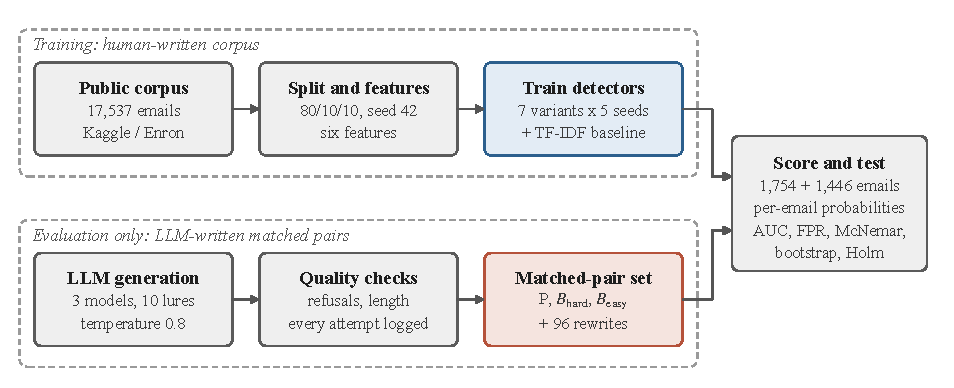
\includegraphics[width=1.0\linewidth]{figures/fig1_workflow.pdf}
\caption{Study design. Detectors are trained only on the conventional corpus; the LLM-written matched-pair set is scored once at the end, together with the corpus test split.}
\end{figure}

\subsection{3.2 Training corpus}

The training data come from a public Kaggle phishing-email collection with the fields ``Email Text'' and ``Email Type'' \cite{subaiey2024}; its legitimate class is dominated by Enron corporate mail \cite{klimt2004}. We removed empty rows and exact duplicate texts, which left 17,537 emails (37.4\% phishing). A stratified 80/10/10 split with seed 42 gave 14,029 training, 1,754 validation and 1,754 test emails; the validation and test splits each hold 656 phishing and 1,098 legitimate messages. The training split was balanced by random oversampling of the phishing class \cite{lemaitre2017}, giving 17,566 rows (8,783 per class). Unlike our earlier pilot, which used a 1,600-row subset, all models here are trained on this full training split.

\subsection{3.3 Matched-pair evaluation set}

The evaluation set is organised around ten attack scenarios: an IT password reset, a chief-executive wire-transfer request, a payment-service account suspension, an HR policy document, a software renewal invoice, a courier delivery failure, a prize notification, a bank login alert, a mailbox-full warning, and a colleague sharing a quarterly report through a cloud drive. For each scenario and generator we requested five kinds of email (Table 2). The two benign conditions are the core of the design. $B_{\mathrm{hard}}$ keeps the sender role, topic and pressure cues of the phishing email but points to a legitimate action through an official channel, such as a password expiry notice that directs the employee to the usual intranet portal. $B_{\mathrm{easy}}$ is an ordinary message on a related topic with no deadline, link or authority appeal. Fig. 2 illustrates one scenario.

\begin{table}[!htbp]
\centering
\footnotesize
\caption{Conditions in the matched-pair set. Counts are accepted emails across three generators.}
\begin{tabularx}{\linewidth}{llYYll}
\toprule
\textbf{Condition} & \textbf{Label} & \textbf{Intent} & \textbf{Surface cues} & \textbf{Register} & \textbf{Emails} \\
\midrule
P & Phishing (1) & Malicious & Deadline, link, authority & As generated & 450 \\
$B_{\mathrm{hard}}$ & Legitimate (0) & Benign & Same as P & As generated & 450 \\
$B_{\mathrm{easy}}$ & Legitimate (0) & Benign & None & As generated & 450 \\
$P_{\mathrm{R}}$ & Phishing (1) & Malicious, unchanged & Unchanged & Rewritten & 48 \\
$B_{\mathrm{hard,R}}$ & Legitimate (0) & Benign, unchanged & Unchanged & Rewritten & 48 \\
\bottomrule
\end{tabularx}
\end{table}

P and $B_{\mathrm{hard}}$ are matched at the level of scenario, sender role and cue set; each is an independent generation, not an edit of the other. The register rewrites are matched at the level of the individual email. For each generator and for each of P and $B_{\mathrm{hard}}$, we sampled eight accepted emails and asked a fixed rewriter model to restate each one in two registers, a terse internal note and a courteous customer-service message, keeping every fact, name, link, number and the sender's intent. This produced 96 rewrites of 48 source emails, 48 rewrites per condition, each linked to its source email. P and $B_{\mathrm{hard}}$ are therefore scenario-matched independent generations, whereas each rewrite is an email-level transformation of one source email; we use ``matched pair'' in the first, scenario-level sense.

\begin{figure}[!htbp]
\centering
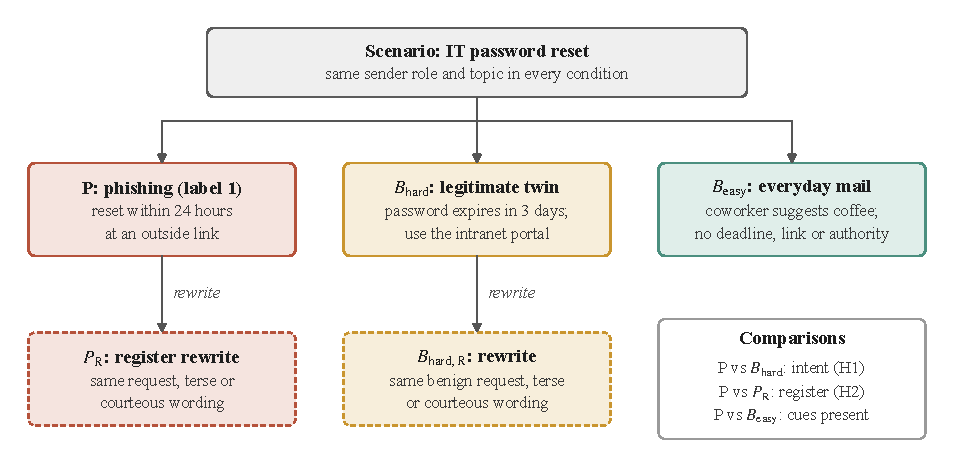
\includegraphics[width=0.92\linewidth]{figures/fig2_design.pdf}
\caption{The matched-pair design for one scenario. P and $B_{\mathrm{hard}}$ share sender role and cues but differ in intent; $P_{\mathrm{R}}$ and $B_{\mathrm{hard,R}}$ change only register. The same structure is repeated for ten scenarios and three generators.}
\end{figure}

\subsection{3.4 Generators and generation protocol}

We used three generators through the Groq API: allam-2-7b \cite{bari2024,groq2025allam}, qwen3.8-27b from the Qwen3 family \cite{yang2025,groq2026qwen}, and gpt-oss-20b \cite{openai2025gptoss}, which also served as the single rewriter. A fourth candidate, gpt-oss-120b, refused 62\% of phishing requests in a pilot and was dropped. All requests used one system prompt that asked for a realistic email for a labelled detector dataset, returned as a subject line and body, with concrete fictional names and no placeholder slots or safety notes. Sampling temperature was 0.8 with a 1,200-token limit. For the two reasoning models, reasoning output was hidden or set to low effort so that it could not consume the token budget.

Each response passed automatic checks. A response was rejected as a refusal if a refusal phrase appeared in its opening and it was short or lacked a subject line, and as too short below ten words. Reasoning blocks were stripped. Template placeholders such as [Name] were flagged rather than rejected, because allam-2-7b produced them in 95\% of its emails across all conditions; since they occur at a similar rate in phishing and benign mail from that generator, the matched design reduces, but does not eliminate, their confounding effect. Every attempt was written to a log with its outcome, so that the selection process can be audited (Table 3). We generated until each generator-condition cell held 150 accepted emails, 15 per scenario.

\begin{table}[!htbp]
\centering
\footnotesize
\caption{Generation attempts by outcome.}
\begin{tabularx}{\linewidth}{Yllllll}
\toprule
\textbf{Generator} & \textbf{Requests} & \textbf{Accepted} & \textbf{Refused} & \textbf{Too short} & \textbf{API error} & \textbf{Refusal rate} \\
\midrule
allam-2-7b & 452 & 450 & 0 & 2 & 0 & 0.0\% \\
qwen3.8-27b & 452 & 450 & 1 & 0 & 1 & 0.2\% \\
gpt-oss-20b & 537 & 450 & 87 & 0 & 0 & 16.2\% \\
gpt-oss-20b (rewrites) & 96 & 96 & 0 & 0 & 0 & 0.0\% \\
\bottomrule
\end{tabularx}
\end{table}

The refusals of gpt-oss-20b are themselves informative. Of its 87 refusals, 50 were phishing requests and 37 were requests for the legitimate twin $B_{\mathrm{hard}}$. The refusal counts suggest that benign prompts containing phishing-like cues may also trigger refusals.

\subsection{3.5 Handcrafted features}

Six features were computed for every email in both test sets and in the training data (Table 4). The behavioural group, named for brevity, contains statistical-text features that describe the text as a statistical object rather than measure behaviour; the psychological group counts persuasion cues described in the phishing literature \cite{ferreira2015,cialdini2006influence}.

\begin{table}[!htbp]
\centering
\footnotesize
\caption{Handcrafted features.}
\begin{tabularx}{\linewidth}{YlY}
\toprule
\textbf{Feature} & \textbf{Group} & \textbf{Computation} \\
\midrule
Perplexity & Behavioural & GPT-2 \cite{radford2019language} perplexity over the first 1,024 tokens, sliding windows with stride 512, capped at 10,000 \\
Grammar-error rate & Behavioural & LanguageTool \cite{languagetool} (en-US) issues per 100 words, numerator and denominator both on the first 1,500 characters \\
Word count & Behavioural & Whitespace-delimited tokens \\
Urgency & Psychological & Regex count of terms such as ``immediately'', ``urgent'', ``within N hours'', ``final notice'' \\
Fear & Psychological & Regex count of terms such as ``suspended'', ``terminated'', ``legal action'', ``unauthorized'' \\
Authority & Psychological & spaCy \cite{honnibal2020spacy} ORG entities in the first 3,000 characters plus a count of titles such as CEO, HR, director, helpdesk \\
\bottomrule
\end{tabularx}
\end{table}

The grammar-error rate in our pilot used a truncated numerator over a full-length denominator. Here both are computed on the same 1,500 characters, so the rate does not shrink with email length.

\subsection{3.6 Models}

All neural variants use the architecture shown in Fig. 3. DistilBERT \cite{sanh2019} processes email text truncated to 512 WordPiece tokens and produces a 768-dimensional representation from the final hidden state of the [CLS] token. For each variant, the selected handcrafted features are standardised with statistics computed on the training split (Eq. 1). The standardised feature vector is concatenated with the DistilBERT representation and passed to a classifier with a fully connected layer of 256 ReLU units, dropout with probability 0.2 and a single-logit output layer, and a sigmoid converts the logit into the predicted phishing probability (Eq. 2):

\begin{equation}
\tilde{s}_j = \frac{s_j - \mu_j}{\sigma_j}, \qquad z = \left[\, h \,;\, \tilde{s} \,\right] \in \mathbb{R}^{768+k}
\end{equation}
\begin{equation}
\hat{y} = \mathrm{sigmoid}\!\left( w_2^{\top}\, \mathrm{Dropout}\big(\mathrm{ReLU}(W_1 z + b_1)\big) + b_2 \right)
\end{equation}

Here \textit{h} is the 768-dimensional [CLS] embedding; \textit{s} holds the \textit{k} handcrafted features selected for the variant (\textit{k} = 0 for the baseline, and 1, 3 or 6 otherwise); \textit{$\mu$} and \textit{$\sigma$} hold the per-feature means and standard deviations on the training split, applied element-wise to each feature \textit{j} in Eq. (1); \textit{z} is the concatenated representation; \textit{W}$_1$ (256 $\times$ (768 + \textit{k})) and \textit{b}$_1$ (256) are the weights and bias of the hidden layer; \textit{w}$_2$ (256) and \textit{b}$_2$ (scalar) are those of the output layer; and \textit{$\hat{y}$} is the predicted phishing probability. Standardisation uses scikit-learn's StandardScaler, which leaves a zero-variance feature unscaled rather than adding a constant to the denominator.

We call this a feature-augmented DistilBERT rather than a dual-stream model, because the features enter by plain concatenation with no separate learned branch. Seven variants differ only in s: baseline (no features); three single behavioural features (perplexity, grammar, length); the behavioural block of all three; the psychological block of urgency, fear and authority; and the full set of six.

\begin{figure}[!htbp]
\centering
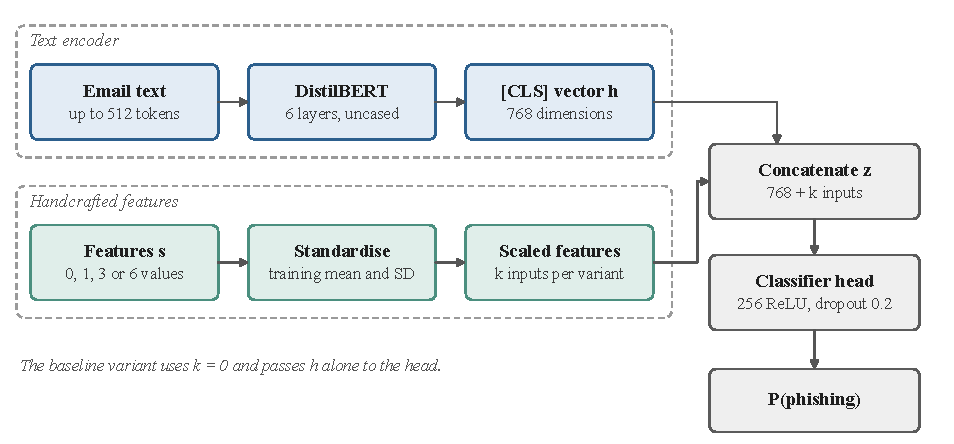
\includegraphics[width=0.92\linewidth]{figures/fig3_architecture.pdf}
\caption{Feature-augmented DistilBERT. The standardised feature vector is appended to the [CLS] embedding before a two-layer head; there is no separate learned feature branch.}
\end{figure}

The lexical baseline is a TF-IDF vectoriser over word unigrams and bigrams (minimum document frequency 2, maximum 0.9, 50,000 features, sublinear term frequency) followed by logistic regression (C = 10, balanced class weights, seed 42) \cite{pedregosa2011}. It is trained on exactly the same training file as DistilBERT, which removes the training-volume mismatch of our pilot.

\subsection{3.7 Training}

Each DistilBERT variant was fine-tuned for three epochs with AdamW \cite{loshchilov2019} (learning rate 2 $\times$ 10$^{-5}$, weight decay 0.01), batch size 16, a linear schedule with 10\% warm-up, gradient clipping at norm 1.0 and binary cross-entropy on logits. The checkpoint with the best validation F1 was kept. Every variant was trained with five seeds (0--4) that fix data order, dropout and head initialisation, for 35 models in total. Training used mixed precision on two NVIDIA T4 GPUs, with the 35 runs split between the two cards. Each training run was assigned to a single GPU, and runs were executed independently.

\subsection{3.8 Hypotheses and analysis plan}

We specified four hypotheses with numerical thresholds before the matched-pair set was scored.

\begin{itemize}
\item \textbf{H1, intent blindness.} Detectors trained on the corpus separate P from $B_{\mathrm{hard}}$ with AUC $\leq$ 0.75, while scoring $\geq$ 0.98 on the corpus test split.
\item \textbf{H2, register sensitivity.} An intent-preserving register rewrite moves DistilBERT scores more than flipping intent (P versus $B_{\mathrm{hard}}$) does.
\item \textbf{H3, features encode authorship.} Perplexity, grammar-error rate and length separate conventional-corpus text from LLM-generated text (AUC > 0.9) but not P from $B_{\mathrm{hard}}$ (AUC < 0.65), and adding them raises recall and $B_{\mathrm{hard}}$ false positives by similar amounts.
\item \textbf{H4, lexical trigger.} TF-IDF has high recall on P but a false-positive rate of at least 40\% on $B_{\mathrm{hard}}$.
\end{itemize}

A fifth hypothesis on pair-contrastive fine-tuning was planned as optional and was not run, under a cut rule fixed in advance.

The primary unit of analysis is the seed ensemble: for each variant and email we average the five seed probabilities and threshold the mean at 0.5, a value fixed in advance and not tuned. Training-run variability is reported separately as the spread of per-seed results. We report recall on phishing conditions, false-positive rate (FPR) on benign conditions, and AUC for separating two conditions \cite{hanley1982}. Precision and F1 are not reported on the matched-pair subsets, because they depend on an arbitrary mix of conditions. Paired model comparisons on the same emails use the exact McNemar test \cite{mcnemar1947,dietterich1998} and a paired bootstrap with 2,000 resamples for differences in recall \cite{efron1993bootstrap}; p-values for the seven planned comparisons against the baseline are adjusted with the Holm procedure \cite{holm1979}. Because emails within a generator-scenario cell are not independent, confidence intervals for AUC use a cluster bootstrap that resamples the 30 cells. Feature effects are summarised with Cohen's d \cite{cohen1988statistical}. These choices follow common guidance on significance testing and run-to-run variance in machine learning \cite{dror2018,bouthillier2021}.

\section{4. Implementation and Reproducibility}

\textbf{Generation procedure.} The pipeline is written in Python with PyTorch \cite{paszke2019} and Hugging Face Transformers \cite{wolf2020}; scikit-learn, pandas and SciPy handle the baseline and the statistics. Generation runs one worker per model, each behind its own rate limiter that reads the provider's remaining-token and reset headers and waits only long enough for the token budget to refill.

\textbf{Computational resources.} Under free-tier limits the 1,446 accepted emails took about 3.5 hours to collect. Feature extraction over the 17,566 training rows took about two hours on a T4 GPU, dominated by LanguageTool. Each training run took about 14 minutes, and the 35 runs finished in about 4.2 hours of wall-clock time on two T4 cards. Scoring all checkpoints on both test sets took about 40 minutes. Table 5 lists the settings a reader needs to repeat the study.

\begin{table}[!htbp]
\centering
\footnotesize
\caption{Reproducibility details.}
\begin{tabularx}{\linewidth}{YY}
\toprule
\textbf{Item} & \textbf{Setting} \\
\midrule
Corpus split & Exact-duplicate removal; stratified 80/10/10, seed 42; random oversampling of the training split, seed 42 \\
Generators & allam-2-7b, qwen3.8-27b, gpt-oss-20b via Groq API, November 2026; prompt version mpg-v1 \\
Rewriter & gpt-oss-20b, two registers (terse internal, courteous customer service) \\
Sampling & Temperature 0.8, maximum 1,200 output tokens; reasoning hidden (Qwen) or low effort (gpt-oss) \\
Acceptance rules & Refusal phrase in opening and short or no subject line; fewer than 10 words; placeholders flagged, not removed \\
Encoders & distilbert-base-uncased, 512 tokens, head 768 + k $\rightarrow$ 256 $\rightarrow$ 1, dropout 0.2; roberta-base with the same head and training settings (Section 5.8) \\
Optimisation & AdamW, lr 2 $\times$ 10$^{-5}$, weight decay 0.01, batch 16, 3 epochs, 10\% warm-up, clip 1.0, mixed precision \\
Model selection & Best validation F1 per run; seeds 0--4 for every variant \\
Lexical baseline & TF-IDF unigrams and bigrams, min\_df 2, max\_df 0.9, 50,000 features, sublinear tf; logistic regression C = 10, balanced, seed 42 \\
Decision threshold & 0.5 on the seed-averaged probability, fixed in advance \\
Statistics & Exact McNemar; paired bootstrap (2,000); cluster bootstrap over 30 generator-scenario cells (2,000); Holm across 7 comparisons \\
Feature tools & GPT-2 (gpt2), LanguageTool 6.8 en-US, spaCy en\_core\_web\_sm \\
Analysis software & scikit-learn 1.9.1, pandas 3.0.5, SciPy 1.18.1, NumPy 2.5.3 \\
\bottomrule
\end{tabularx}
\end{table}

The repository (github.com/devarshganatra/ai-phishing) contains the generation harness and its attempt log, feature extraction, training and scoring scripts, the per-email prediction files, and the scripts that produce every table and figure in this paper.

\section{5. Results}

\subsection{5.1 In-distribution performance}

On the conventional test split, all eight models achieved near-ceiling performance with small between-model differences (Table 6). DistilBERT F1 ranged from 0.985 to 0.987 and ROC-AUC from 0.9994 to 0.9995, with seed standard deviations of 0.004 or less. No handcrafted feature changed in-distribution performance by more than the seed-to-seed variation. The TF-IDF baseline matched the encoders on F1 (0.987) with a slightly lower AUC (0.9985).

\begin{table}[!htbp]
\centering
\footnotesize
\caption{Conventional test split (n = 1,754). DistilBERT values are mean $\pm$ SD over five seeds; TF-IDF is deterministic.}
\begin{tabularx}{\linewidth}{Ylll}
\toprule
\textbf{Model} & \textbf{F1} & \textbf{Recall} & \textbf{ROC-AUC} \\
\midrule
DistilBERT baseline & 0.987 $\pm$ 0.001 & 0.985 $\pm$ 0.004 & 0.9994 $\pm$ 0.0002 \\
+ perplexity & 0.986 $\pm$ 0.002 & 0.984 $\pm$ 0.004 & 0.9994 $\pm$ 0.0001 \\
+ grammar & 0.987 $\pm$ 0.001 & 0.985 $\pm$ 0.001 & 0.9994 $\pm$ 0.0001 \\
+ length & 0.985 $\pm$ 0.004 & 0.983 $\pm$ 0.006 & 0.9994 $\pm$ 0.0002 \\
+ behavioural (3) & 0.987 $\pm$ 0.002 & 0.987 $\pm$ 0.003 & 0.9994 $\pm$ 0.0001 \\
+ psychological (3) & 0.987 $\pm$ 0.003 & 0.986 $\pm$ 0.004 & 0.9995 $\pm$ 0.0001 \\
+ full (6) & 0.987 $\pm$ 0.002 & 0.984 $\pm$ 0.003 & 0.9995 $\pm$ 0.0002 \\
TF-IDF + logistic regression & 0.987 & 0.985 & 0.9985 \\
\bottomrule
\end{tabularx}
\end{table}

\subsection{5.2 Degradation on matched pairs (RQ1)}

On the matched-pair phishing emails, performance declined substantially (Fig. 4). The seed-ensembled baseline detected 52.7\% of P emails, against 98.5\% of phishing in the conventional test split, a loss of 46 percentage points. No DistilBERT variant exceeded 58.4\%.

\begin{figure}[!htbp]
\centering
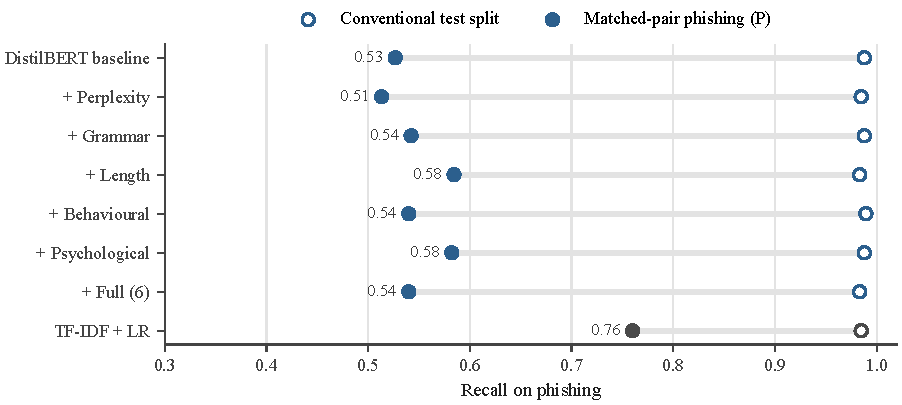
\includegraphics[width=1.0\linewidth]{figures/fig4_collapse.pdf}
\caption{Phishing recall on the conventional test split (open circles) and on the 450 matched-pair phishing emails (filled circles), seed-ensembled. Every model loses at least 22 points; the DistilBERT variants lose 40 to 47.}
\end{figure}

Training-run variance also changed scale. Across seeds, conventional recall for the baseline varied with a standard deviation of 0.004; recall on P varied with a standard deviation of 0.129, about 35 times larger (per-seed mean 0.545). The other variants showed seed standard deviations between 0.058 and 0.141 on P. A single training run, as in our pilot and much prior work, could therefore have changed the apparent ranking of the variants.

The loss also depended on the generator. The baseline detected 74.0\% of phishing written by allam-2-7b, 40.7\% from gpt-oss-20b and 43.3\% from qwen3.8-27b. As Section 5.3 shows, the higher figure for allam-2-7b does not mean better discrimination: the same model also flagged 62\% of allam-2-7b's legitimate twins.

\subsection{5.3 Can the detectors separate intent? (RQ2, H1)}

Table 7 reports the central result. Every DistilBERT variant separated phishing from its legitimate twin with an AUC between 0.615 and 0.632, and the cluster-bootstrap intervals of all seven variants overlap almost entirely. The same models separated phishing from plain legitimate mail with an AUC of about 0.78 to 0.80. This gap of roughly 0.17 AUC suggests that phishing-like cues influence the predictions even when the request is legitimate: a legitimate email with a deadline, a link and an authority figure was scored much like phishing (Fig. 5). Because P and $B_{\mathrm{hard}}$ were generated independently, the gap cannot be attributed to intent alone. Per-seed AUCs for the baseline ranged only from 0.607 to 0.647, so this result is stable across training runs.

\begin{table}[!htbp]
\centering
\footnotesize
\caption{Matched-pair results on seed-ensembled predictions. Recall on phishing conditions, FPR on benign conditions; AUC 95\% intervals from a cluster bootstrap over 30 generator-scenario cells.}
\begin{tabularx}{\linewidth}{YlllYl}
\toprule
\textbf{Model} & \textbf{Recall P} & \textbf{FPR $B_{\mathrm{hard}}$} & \textbf{FPR $B_{\mathrm{easy}}$} & \textbf{AUC P vs $B_{\mathrm{hard}}$ [95\% CI]} & \textbf{AUC P vs $B_{\mathrm{easy}}$} \\
\midrule
DistilBERT baseline & 0.527 & 0.369 & 0.116 & 0.617 [0.567, 0.684] & 0.783 \\
+ perplexity & 0.513 & 0.347 & 0.098 & 0.620 [0.568, 0.689] & 0.788 \\
+ grammar & 0.542 & 0.353 & 0.111 & 0.626 [0.574, 0.695] & 0.783 \\
+ length & 0.584 & 0.400 & 0.098 & 0.617 [0.567, 0.683] & 0.794 \\
+ behavioural (3) & 0.540 & 0.382 & 0.109 & 0.616 [0.563, 0.685] & 0.787 \\
+ psychological (3) & 0.582 & 0.429 & 0.131 & 0.615 [0.566, 0.679] & 0.789 \\
+ full (6) & 0.540 & 0.362 & 0.100 & 0.632 [0.579, 0.705] & 0.797 \\
TF-IDF + logistic regression & 0.760 & 0.407 & 0.162 & 0.749 [0.686, 0.820] & 0.859 \\
\bottomrule
\end{tabularx}
\end{table}

The false-positive rates tell the same story from the other side. The baseline flagged 36.9\% of $B_{\mathrm{hard}}$ emails but 11.6\% of $B_{\mathrm{easy}}$ emails, a 3.2-fold difference associated with the matched-cue condition. By generator, the baseline flagged 62.0\% of allam-2-7b's legitimate twins, 30.0\% of gpt-oss-20b's and 18.7\% of qwen3.8-27b's; its AUC for P against $B_{\mathrm{hard}}$ was 0.59, 0.61 and 0.68 for the three generators. Since 0.62 is far below the pre-specified ceiling of 0.75 while test-split AUC is 0.999, H1 is supported.

\textbf{Label audit.} Because the twin labels follow from the generation prompts, two annotators independently judged a blinded sample of 90 emails: 60 $B_{\mathrm{hard}}$ twins (two from every generator-scenario cell), 20 P and 10 $B_{\mathrm{easy}}$, shuffled and stripped of condition, generator and scenario. For each email they gave a verdict (phishing, legitimate or cannot tell) and a suspicion rating from 1 to 5. Their verdicts matched the intended labels for 86.7\% and 87.8\% of emails, and they agreed with each other on 81.1\% (Cohen's $\kappa$ = 0.55). Both annotators judged 48 of the 60 twins (80.0\%) legitimate, both judged 3 (5.0\%) phishing, and they split on the remaining 9. Mean suspicion was 4.17 for P, 2.04 for $B_{\mathrm{hard}}$ and 1.95 for $B_{\mathrm{easy}}$, so the twins read close to ordinary legitimate mail despite carrying the cues of phishing. Restricting $B_{\mathrm{hard}}$ to the 48 twins both annotators judged legitimate left the result unchanged: AUC for P against $B_{\mathrm{hard}}$ was 0.603 for the DistilBERT baseline (0.613 on all 60 audited twins), 0.651 for RoBERTa (Section 5.8) and 0.737 for TF-IDF. A minority of ambiguous twins therefore does not explain the low AUC.

\begin{figure}[!htbp]
\centering
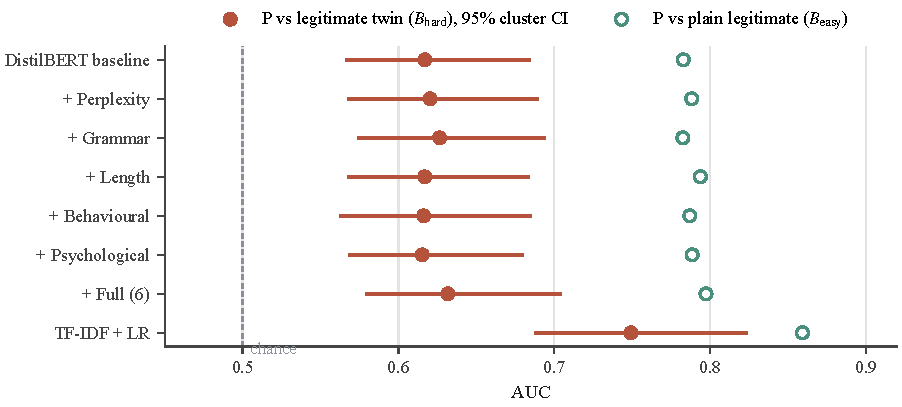
\includegraphics[width=1.0\linewidth]{figures/fig5_intent_auc.pdf}
\caption{AUC for separating phishing from its legitimate twin (filled, with 95\% cluster-bootstrap intervals) and from plain legitimate mail (open). The dashed line marks chance. All DistilBERT variants fall to about 0.62 once the cues are matched.}
\end{figure}

\subsection{5.4 Does register move the scores? (RQ3, H2)}

We measured the effect of register on the 48 pairs that link a rewrite to its source email. Rewriting changed the baseline's phishing probability by 0.124 on average in absolute terms. Flipping intent, measured as the absolute difference between the mean scores of P and $B_{\mathrm{hard}}$ within each generator-scenario cell, changed it by 0.200. The same ordering held for the behavioural variant (0.109 against 0.194), the full variant (0.140 against 0.214) and TF-IDF (0.122 against 0.280).

On the paired emails the direction of the register effect was not consistent. The 24 phishing emails selected for rewriting were harder than average (37.5\% detected by the baseline), and their rewrites were detected slightly more often (43.8\%; exact McNemar p = 0.25). Comparing all 450 P emails with the 48 rewrites would suggest a drop from 52.7\% to 43.8\%, but that difference comes from which emails were sampled, not from the rewriting. Register therefore moves individual scores by a noticeable amount in both directions, but less than intent does, and H2 is not supported. Rewritten legitimate twins were flagged at about the same rate as the originals (37.5\% against 36.9\%).

\subsection{5.5 What the handcrafted features measure (RQ4, H3)}

Table 8 tests each feature as a stand-alone separator. Grammar-error rate and perplexity separated conventional-corpus text from LLM-generated text very well (AUC 0.964 and 0.889) but barely separated phishing from its twin within LLM text (0.567 and 0.519). Their spread across generators within the phishing condition was large, 1.3 standard deviations, while their difference between P and $B_{\mathrm{hard}}$ was small (Cohen's d of $-$0.26 and 0.08). The urgency and fear counts behaved in the opposite way: they carried a real intent signal (AUC 0.773 and 0.683, d = 1.08 and 0.84) and almost no generator signal.

Tested one at a time, none of the three psychological counts separated phishing from legitimate mail in the training corpus (AUC 0.43--0.51), so they were not cues the detectors could have learned there. On the matched pairs, authority was balanced between P and $B_{\mathrm{hard}}$ as designed (AUC 0.49, for both its job-title and organisation-name parts), whereas urgency and fear words remained more frequent in phishing than in its twins. Normalising the counts per 100 words left these conclusions unchanged (urgency AUC 0.786, fear 0.686), and word count itself was matched (AUC 0.51). The twins therefore hold authority and length constant but not the full intensity of urgency and fear language. This works against our conclusion rather than for it: a residual cue difference should make P easier to separate from $B_{\mathrm{hard}}$, yet the encoders still reached only 0.62.

\begin{table}[!htbp]
\centering
\footnotesize
\caption{Each feature as a stand-alone separator. AUC is reported direction-free, as max(AUC, 1 $-$ AUC), so 0.5 means no separation in either direction. Generator spread = range of generator means within P, in pooled SD units.}
\begin{tabularx}{\linewidth}{YYlYY}
\toprule
\textbf{Feature} & \textbf{AUC corpus vs LLM} & \textbf{AUC P vs $B_{\mathrm{hard}}$} & \textbf{Cohen's d, P vs $B_{\mathrm{hard}}$} & \textbf{Generator spread (SD)} \\
\midrule
Perplexity & 0.889 & 0.519 & 0.08 & 1.34 \\
Grammar-error rate & 0.964 & 0.567 & $-$0.26 & 1.32 \\
Word count & 0.537 & 0.513 & $-$0.02 & 1.59 \\
Urgency & 0.680 & 0.773 & 1.08 & 0.07 \\
Fear & 0.568 & 0.683 & 0.84 & 0.07 \\
Authority & 0.809 & 0.513 & $-$0.15 & 0.68 \\
\bottomrule
\end{tabularx}
\end{table}

The feature distributions help explain why the tested behavioural-feature configurations did not improve discrimination (Fig. 6). In the training corpus, legitimate and phishing emails had median perplexities of 52 and 89 and median grammar-error rates of 20.7 and 22.1 issues per 100 words. LLM-written emails sat far outside that range in both conditions: median perplexity was 17.8 for P and 17.5 for $B_{\mathrm{hard}}$, and median grammar-error rate was 0.84 and 1.14. Seen through these features, all LLM mail looks alike, and none of it resembles the phishing the model was trained on.

\begin{figure}[!htbp]
\centering
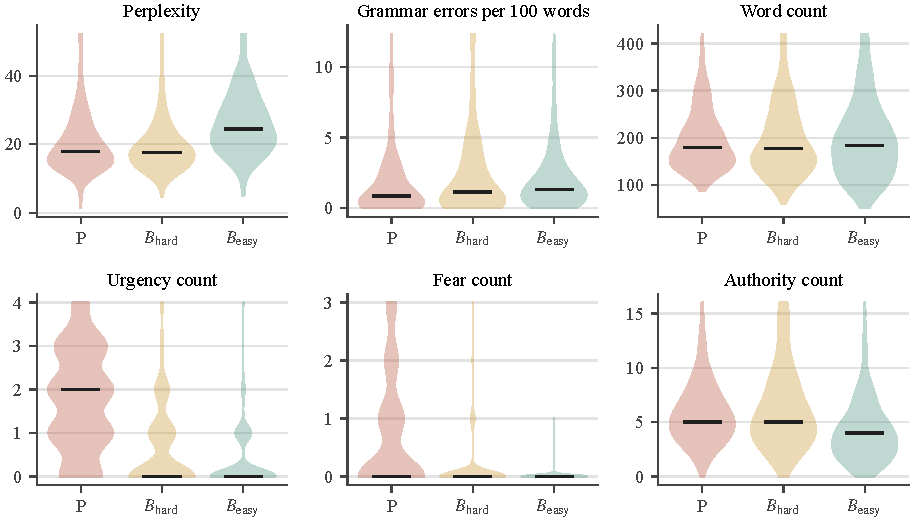
\includegraphics[width=1.0\linewidth]{figures/fig6_features.pdf}
\caption{The six handcrafted features in the P, $B_{\mathrm{hard}}$ and $B_{\mathrm{easy}}$ conditions. Perplexity, grammar-error rate, word count and authority overlap almost completely between P and $B_{\mathrm{hard}}$; urgency and fear do not.}
\end{figure}

Adding the features to DistilBERT confirmed this (Table 9, Fig. 7). Perplexity, grammar-error rate, the behavioural block and the full set changed recall on P by between $-$1.3 and +1.6 points, none significant after Holm correction. Length and the psychological block raised recall by 5.8 and 5.6 points (Holm-adjusted p < 0.001), but they also raised the false-positive rate on $B_{\mathrm{hard}}$, by 3.1 and 6.0 points, and left AUC for P against $B_{\mathrm{hard}}$ unchanged (0.617 and 0.615). These two variants moved the decision threshold rather than improving discrimination. H3 is therefore only partially supported. Grammar-error rate meets both thresholds; perplexity separates P from $B_{\mathrm{hard}}$ as poorly as predicted but falls just short of the 0.9 threshold for separating the corpus from LLM text (0.889); and length meets neither condition, although adding it raised recall and $B_{\mathrm{hard}}$ false positives together, as the hypothesis predicted.

\begin{table}[!htbp]
\centering
\footnotesize
\caption{Each variant against the baseline on the 450 P emails (paired). Bootstrap 95\% CI for the recall difference; exact McNemar with Holm adjustment across seven comparisons. ``Only variant / only baseline'' are the discordant detection counts: P emails detected by the variant but not by the baseline, and the reverse.}
\begin{tabularx}{\linewidth}{llYYll}
\toprule
\textbf{Variant} & \textbf{Recall} & \textbf{$\Delta$ recall [95\% CI]} & \textbf{Only variant / only baseline} & \textbf{McNemar p} & \textbf{Holm p} \\
\midrule
TF-IDF & 0.760 & +0.233 [0.193, 0.276] & 107 / 2 & < 0.001 & < 0.001 \\
+ length & 0.584 & +0.058 [0.036, 0.082] & 28 / 2 & < 0.001 & < 0.001 \\
+ psychological & 0.582 & +0.056 [0.036, 0.078] & 25 / 0 & < 0.001 & < 0.001 \\
+ grammar & 0.542 & +0.016 [$-$0.004, 0.038] & 14 / 7 & 0.189 & 0.757 \\
+ behavioural & 0.540 & +0.013 [$-$0.004, 0.033] & 12 / 6 & 0.238 & 0.757 \\
+ full & 0.540 & +0.013 [$-$0.007, 0.033] & 13 / 7 & 0.263 & 0.757 \\
+ perplexity & 0.513 & $-$0.013 [$-$0.033, 0.007] & 8 / 14 & 0.286 & 0.757 \\
\bottomrule
\end{tabularx}
\end{table}

\begin{figure}[!htbp]
\centering
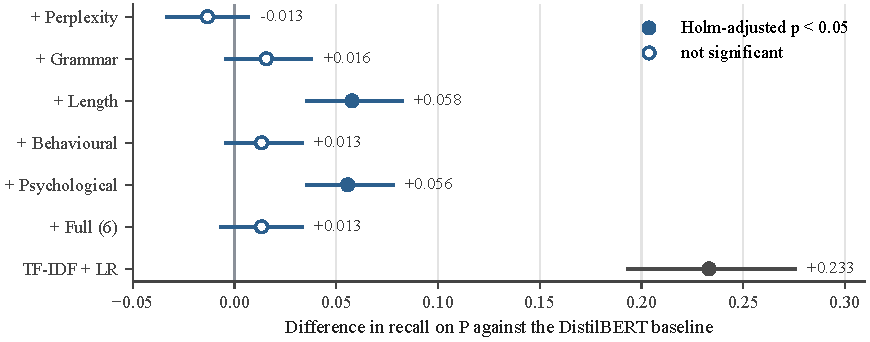
\includegraphics[width=1.0\linewidth]{figures/fig7_forest.pdf}
\caption{Difference in recall on P against the DistilBERT baseline, with paired-bootstrap 95\% intervals. Filled markers denote Holm-adjusted p < 0.05 (exact McNemar); open markers are not significant. Only TF-IDF, length and the psychological block clear zero, and the last two do so by moving the threshold (Table 7).}
\end{figure}

\subsection{5.6 The lexical baseline (RQ5, H4)}

The TF-IDF model detected 76.0\% of P emails and 68.8\% of the rewrites, and it separated P from $B_{\mathrm{hard}}$ with an AUC of 0.749. Its interval [0.686, 0.820] does not overlap the baseline's, so the lexical model achieved higher intent-discrimination AUC than the DistilBERT baseline on this evaluation set. Against the baseline it caught 107 phishing emails that DistilBERT missed and missed only 2 that DistilBERT caught. Its advantage was not bought with training volume. In a learning curve on the conventional test split, its recall was already 0.982 with 1,600 training emails and 0.985 with all 17,566.

Two observations qualify this advantage. First, the lexical model also raised false alarms: it flagged 40.7\% of legitimate twins and 16.2\% of plain legitimate mail, the highest rates of any model, which meets the pre-specified H4 threshold of 40\%, if narrowly. Second, its strongest weights point to corpus provenance (Fig. 8). Apart from function words, the fifteen terms most indicative of legitimate mail include enron, vince, louise, 2000, 2001, 2002, edu and university, which identify the Enron collection and its period. The fifteen most indicative of phishing include click here, remove, viagra, money, free, 2004 and 2005, which identify the spam archives of the mid-2000s. The model learned where an email came from as well as what it asks for, which agrees with the cross-corpus findings of Bhuiyan and Bhuiyan \cite{bhuiyan2026}.

To test how much of the matched-pair result depends on these tokens, we retrained the lexical model under controlled masking, applied identically to training and evaluation text (Table 10). Removing provenance artefacts (digits, URLs, e-mail addresses, reply headers and Enron-specific names) changed AUC for P against $B_{\mathrm{hard}}$ only from 0.749 to 0.741 and test F1 from 0.987 to 0.983. Removing in addition the 200 unigrams with the largest coefficients lowered AUC to 0.726 and the $B_{\mathrm{hard}}$ false-positive rate from 40.9\% to 32.4\%, and removing the urgency, fear and authority lexicons instead gave 0.733 and 38.9\%. The lexical model's intent signal therefore does not rest on provenance tokens, but its false-alarm rate is sensitive to the vocabulary it is allowed to use, and H4 holds only narrowly and not under masking.

\begin{table}[!htbp]
\centering
\footnotesize
\caption{TF-IDF + logistic regression retrained under lexical masking (M1: provenance tokens removed; M2: M1 plus the 200 highest-weight unigrams; M3: M1 plus the urgency, fear and authority lexicons).}
\begin{tabularx}{\linewidth}{Ylllll}
\toprule
\textbf{Condition} & \textbf{Test F1} & \textbf{Recall P} & \textbf{FPR $B_{\mathrm{hard}}$} & \textbf{AUC P vs $B_{\mathrm{hard}}$} & \textbf{E-PhishLLM F1} \\
\midrule
M0 none & 0.987 & 0.762 & 0.409 & 0.749 & 0.699 \\
M1 provenance removed & 0.983 & 0.718 & 0.393 & 0.741 & 0.688 \\
M2 + top-200 tokens & 0.968 & 0.676 & 0.324 & 0.726 & 0.673 \\
M3 + cue lexicons & 0.983 & 0.713 & 0.389 & 0.733 & 0.670 \\
\bottomrule
\end{tabularx}
\end{table}

\begin{figure}[!htbp]
\centering
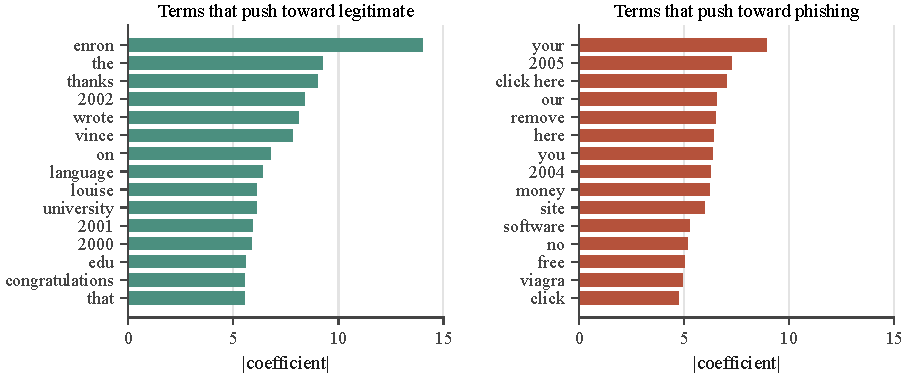
\includegraphics[width=0.96\linewidth]{figures/fig8_tfidf_terms.pdf}
\caption{The fifteen strongest TF-IDF terms for each class, by absolute coefficient. Legitimate-class terms name the Enron collection and its years; phishing-class terms come from mid-2000s spam.}
\end{figure}

\subsection{5.7 Scenario-level blind spots}

Recall differed far more across scenarios than across models (Fig. 9). Both the baseline and TF-IDF detected nearly every payment-service suspension and prize email (100\% each) and almost every bank login alert (95.6\% and 100\%). Both failed on the two lures that most resemble everyday workplace mail. On the HR policy document, the baseline and TF-IDF each detected 8.9\%. On the colleague sharing a quarterly report through a cloud drive, they detected 2.2\% and 13.3\%. TF-IDF's lead over the encoder came from five scenarios: the courier notice (91.1\% against 24.4\%), the mailbox-full warning (91.1\% against 33.3\%), the invoice (91.1\% against 55.6\%), the wire transfer (64.4\% against 33.3\%) and the password reset (100\% against 73.3\%). These are the lures that most resemble mass-mailed templates, which fits the provenance reading above, although we did not test that explanation directly.

\begin{figure}[!htbp]
\centering
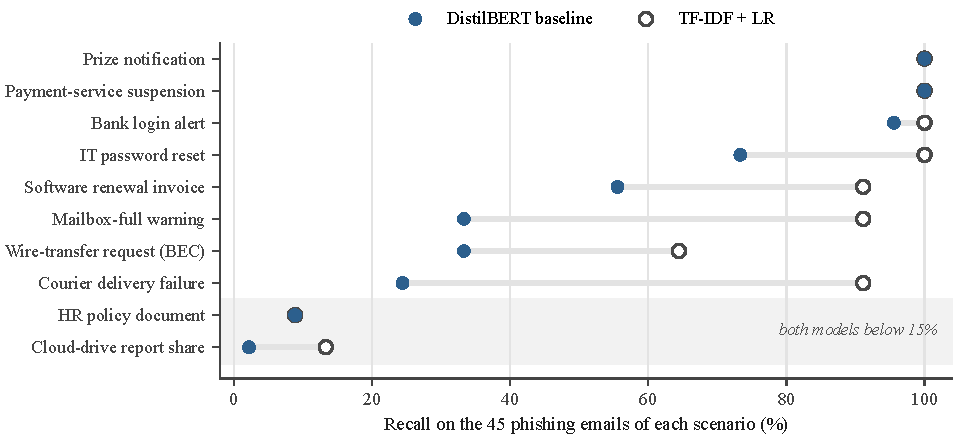
\includegraphics[width=1.0\linewidth]{figures/fig9_scenarios.pdf}
\caption{Recall by attack scenario for the seed-ensembled DistilBERT baseline (filled) and TF-IDF (ring), 45 phishing emails per scenario across three generators. The shaded rows are the two workplace lures that both models miss.}
\end{figure}

\subsection{5.8 A stronger encoder and an external benchmark}

To check that the result is not specific to DistilBERT, we fine-tuned RoBERTa-base \cite{liu2019} with the same data, five seeds and threshold, and repeated the DistilBERT baseline in the same environment. The repeat reproduced the reported run (recall 0.529 against 0.527, McNemar p = 1.0). RoBERTa matched the other models in distribution (F1 0.987, AUC 0.999) and separated P from $B_{\mathrm{hard}}$ somewhat better, with an AUC of 0.680 [0.627, 0.749], still below the H1 ceiling and below TF-IDF (Fig. 10a). It was also far more conservative: it detected 40.0\% of P and flagged 16.0\% of $B_{\mathrm{hard}}$, both significantly lower than the DistilBERT baseline (Holm-adjusted McNemar p < 0.001). A larger encoder therefore trades recall for fewer false alarms rather than recognising intent, and H1 holds for both encoder families.

We also scored all models on the English portion of E-PhishLLM \cite{pajola2025} (11,502 emails, 52\% phishing), which none of them saw in training. F1 was 0.541 for DistilBERT, 0.573 for RoBERTa and 0.698 for TF-IDF, with AUCs of 0.673, 0.700 and 0.768 (Fig. 10b). These values lie within the range the benchmark's authors report for detectors trained on older corpora, and they reproduce the ordering seen on our matched pairs: the lexical model ahead of both encoders, and RoBERTa ahead of DistilBERT on ranking but with low recall (0.42). The degradation we measure is therefore not an artefact of our generators or prompts.

\begin{figure}[!htbp]
\centering
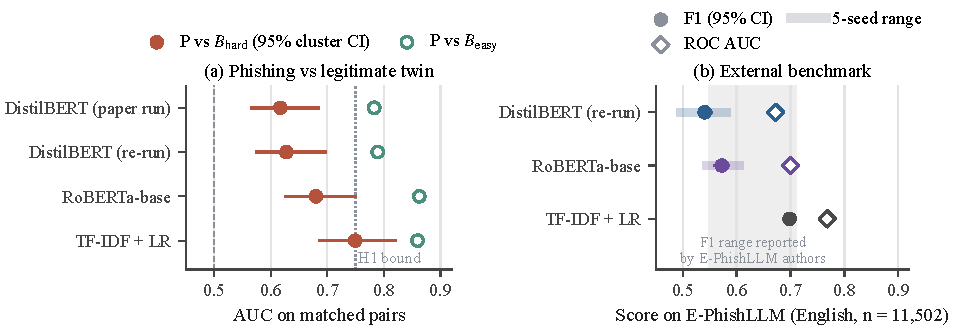
\includegraphics[width=1.0\linewidth]{figures/fig10_baselines.pdf}
\caption{(a) AUC for P against $B_{\mathrm{hard}}$ (filled, 95\% cluster-bootstrap interval) and against $B_{\mathrm{easy}}$ (open) for the DistilBERT baseline, its repeat, RoBERTa-base and TF-IDF; the dotted line marks the H1 ceiling of 0.75. (b) F1 (95\% bootstrap interval; shaded bar, range over five seeds) and ROC AUC on E-PhishLLM. The grey band is the F1 range reported by the benchmark's authors.}
\end{figure}

\section{6. Discussion}

\subsection{6.1 Answers to the research questions}

Table 11 summarises the pre-specified tests. Three of the four hypotheses held, one of them only in part and one narrowly, and the register hypothesis failed.

\begin{table}[!htbp]
\centering
\footnotesize
\caption{Pre-specified hypotheses and outcomes.}
\begin{tabularx}{\linewidth}{YYYY}
\toprule
\textbf{Hypothesis} & \textbf{Pre-specified criterion} & \textbf{Observed} & \textbf{Verdict} \\
\midrule
H1 intent blindness & AUC(P vs $B_{\mathrm{hard}}$) $\leq$ 0.75 with test AUC $\geq$ 0.98 & 0.615--0.632 for all DistilBERT variants; test AUC 0.999 & Supported \\
H2 register sensitivity & Register shift > intent shift & Mean shift 0.124 against 0.200 (baseline); no consistent direction (p = 0.25) & Not supported \\
H3 features encode authorship & Corpus vs LLM AUC > 0.9 and P vs $B_{\mathrm{hard}}$ AUC < 0.65 & Grammar 0.964 / 0.567; perplexity 0.889 / 0.519; length 0.537 / 0.513 & Partly supported \\
H4 lexical trigger & TF-IDF FPR on $B_{\mathrm{hard}}$ $\geq$ 0.40 & 0.407 with recall 0.760; 0.324--0.393 under lexical masking & Supported (narrowly; not robust) \\
\bottomrule
\end{tabularx}
\end{table}

\textbf{RQ1.} The degradation is large and real. Recall on phishing fell from 98.5\% on the conventional split to 52.7\% on matched LLM phishing for the baseline, and no variant passed 58.4\%. The drop varied by generator (74.0\% to 40.7\%), and recall on LLM phishing was about 35 times more variable across seeds than recall in distribution. Rankings of feature variants built on a single seed should not be trusted on shifted data.

\textbf{RQ2.} The encoders barely recognise intent once surface cues are held constant. An AUC of 0.62 between phishing and its legitimate twin means that a randomly chosen phishing email outranks a randomly chosen twin only 62\% of the time. This suggests that much of what looked like phishing detection reflects the cues that typically accompany phishing in the training data.

\textbf{RQ3.} Register is not the main driver. Rewriting a phishing email into another register moved its score by about 0.12 on average, in either direction, while flipping intent moved the cell mean by about 0.20. The encoders are not intent-blind because they are register-bound. They are intent-poor because cue words carry most of their decision. This negative result narrows the explanation. It also argues against simple fixes that normalise style or paraphrase inputs before classification.

\textbf{RQ4.} The behavioural features track corpus and generator differences, not intent. Grammar-error rate and perplexity separated the conventional corpus from LLM-generated text almost perfectly, but their values for phishing and legitimate twins were nearly identical, so they cannot teach a classifier anything about phishing on LLM mail. This matches the finding that perplexity tracks writing style more than authorship \cite{liang2023}, and the fragility of likelihood signals under paraphrase \cite{sadasivan2023,krishna2023}. The psychological counts do carry intent information (d $\approx$ 1 for urgency), as Shahriar et al. reported with learned trait scores \cite{shahriar2022}. Concatenating them to the [CLS] vector shifted the decision threshold but did not improve ranking. The encoder appears to see the same cue words already, and a three-number summary of them adds no new ordering.

\textbf{RQ5.} The lexical baseline achieved higher intent-discrimination AUC than the encoders on this set (0.75 against 0.62 for DistilBERT and 0.68 for RoBERTa), and masking provenance tokens barely changed it (Table 10). Part of the reason is that its vocabulary includes the action words of phishing requests, which a bag-of-words model weighs directly. Its learned weights also encode corpus identity, and it flagged 41\% of legitimate twins. Its advantage is partly real and partly a higher willingness to say ``phishing''.

\subsection{6.2 Why the lexical model separates intent better: a hypothesis}

We offer a hypothesis for the gap between the two model families rather than an explanation. One account is that the encoder pools the whole email into one vector shaped by Enron's corporate register, so that a fluent, polite LLM email is pulled toward the legitimate class regardless of its request. The lexical model has no such pooling. A phrase like ``click here'' adds the same weight whatever the surrounding prose. This account fits the per-generator pattern: the encoder did worst on gpt-oss-20b and qwen3.8-27b and best on allam-2-7b, the only generator whose emails almost always contain template placeholders typical of mass mailings (95\% of its emails, against 3.5\% and 1.5\%). It also fits the scenario pattern, where the lexical model's advantage was concentrated in lures that resemble mass-mailed templates. Our results are consistent with this account but do not establish it; a representation-level probe of the encoder is required to test it.

\subsection{6.3 Relation to prior work}

Our findings extend earlier evaluations of phishing detectors under distribution shift by testing how they respond to legitimate messages that carry phishing-associated cues. SpearBot showed that detectors trained on legacy corpora fail on adversarially refined LLM phishing \cite{qi2025}. We find a large drop without any adversarial refinement, and on scenario-matched pairs the encoders were close to chance. E-PhishGen documented degradation on a large synthetic benchmark \cite{pajola2025}, and our models degraded on it in the same order as on our set (Section 5.8). Our controlled conditions suggest that the degradation reflects sensitivity to phishing-associated cues, although dataset and generation effects cannot be fully separated, and the benign twins expose a false-alarm cost that a phishing-only set cannot show. Bhuiyan and Bhuiyan found that lexical classifiers learn corpus identity across classical datasets \cite{bhuiyan2026}. We see the same provenance tokens in our training corpus, and we add that the lexical model still separates intent better than a fine-tuned encoder. Finally, the design transfers contrast-set \cite{gardner2020} and counterfactual \cite{kaushik2020} evaluation to phishing, where the natural label-flipping edit is a legitimate email that keeps the cues of the attack. The design does not fully isolate authorship, corpus provenance and style; separating them requires further controlled experiments.

\subsection{6.4 Practical implications}

A detector that scores 0.999 AUC on a public corpus may still flag a third of legitimate workplace mail that mentions a deadline and a link, and miss most phishing that looks like an ordinary document share. Neither fact is visible in a phishing-only test set. We suggest five practices for evaluating detectors against LLM-era phishing.

\begin{enumerate}
\item Pair every phishing test email with a legitimate twin that keeps its cues, and report AUC and false-positive rate on the pairs, not only recall.
\item Train with several seeds and report the spread on the shifted set, since it can be an order of magnitude larger than in distribution.
\item Report results by generator and by scenario. Aggregate recall hid both a near-zero scenario and a generator whose higher recall came with a 62\% false-alarm rate.
\item Include a lexical baseline trained on the same split, and inspect its strongest weights for corpus provenance.
\item Log every generation attempt, including refusals, because generators refuse benign twins as well as phishing and the retained set is shaped by those choices.
\end{enumerate}

For defence, the results point away from style features and toward signals that do not depend on how an email is written. Reference-based checks of the sender's claimed identity \cite{liu2025} and LLM judges that reason about the request itself \cite{koide2025} may offer complementary evidence for distinguishing a real policy update from a fake one, although we did not test them here.

\section{7. Limitations and Threats to Validity}

\textbf{Generators.} The matched-pair set uses three generators served by one provider. That supports claims about these models, not about LLM phishing in general, and a broader study would need more model families, including frontier and agentic systems.

\textbf{Construction of the twins.} P and $B_{\mathrm{hard}}$ were generated independently from paired prompts, not produced by editing one email into the other, so they can differ in ways beyond intent. Their labels follow from the prompts. A blinded audit by two annotators (Section 5.3) found that 80\% of sampled twins read as legitimate to both and 5\% as phishing to both, with moderate inter-annotator agreement ($\kappa$ = 0.55), and excluding the disputed twins did not change H1. The audit covered 60 of 450 twins and two annotators, so it bounds rather than eliminates label noise.

\textbf{Authorship and provenance.} The training corpus is conventional public mail and the evaluation emails are LLM-generated, so authorship is confounded with corpus origin, period and topic. Our claims therefore concern intent discrimination within LLM-generated mail; we do not claim that the detectors fail because the text is machine-written. Testing that would require human-written phishing and benign emails matched to the same scenarios.

\textbf{Register test.} The register comparison rests on 96 rewrites of 48 source emails (48 rewrites of 24 emails per condition) produced by a single rewriter, so H2 was tested with low power. A larger, multi-rewriter set could detect a smaller register effect than we can exclude here.

\textbf{Scope of the detectors.} We studied fine-tuned DistilBERT, RoBERTa-base and one lexical model trained on one public corpus, and validated them on one external benchmark, E-PhishLLM \cite{pajola2025}. Larger encoders such as DeBERTa \cite{he2021}, LLM judges \cite{koide2025} and reference-based systems \cite{liu2025} were not evaluated. All emails are English text bodies without headers, URLs that resolve, or attachments.

\textbf{Analysis choices.} The decision threshold was fixed at 0.5 and not recalibrated for the shifted set, which affects recall and false-positive rates but not AUC. The psychological features are keyword and entity counts rather than validated measures, and the twins match authority and length but carry fewer urgency and fear words than the phishing emails (Section 5.5). The hypotheses were recorded in the project repository before scoring, not in a public registry.

\textbf{Reproducibility and dual use.} Hosted models change and are retired, so exact regeneration may not be possible later; the retained emails and the attempt log are the stable record. The phishing emails are dual-use material and are shared only for defensive research under access controls.

\section{8. Conclusion and Future Work}

We asked what phishing detectors respond to when the attacker is an LLM. The matched-condition evaluation provided evidence about how sensitive these detectors are to phishing intent. Fine-tuned DistilBERT classifiers that reached 0.999 AUC on a public corpus separated LLM-written phishing from legitimate emails carrying the same cues with an AUC of only 0.62, and they flagged more than a third of those legitimate emails. The result held across five seeds, three generators and seven feature configurations. Perplexity and grammar-error features, often proposed for LLM-era detection, distinguished the conventional corpus from LLM-generated text but not phishing from legitimate mail, and adding them did not help. Register mattered less than we had expected. A lexical baseline read intent better than the encoder but relied partly on corpus provenance and raised false alarms on 41\% of the twins. Both model families missed nearly every document-sharing lure. RoBERTa-base and an external benchmark, E-PhishLLM, showed the same pattern, and a blinded label audit left the result unchanged.

High performance on the conventional corpus did not predict performance on the matched LLM-generated evaluation set. We recommend that evaluations of phishing detectors include benign controls matched on cues, multiple training seeds, and results broken down by generator and scenario.

Several directions follow. The first is training on contrastive pairs, in which the detector sees phishing and legitimate twins side by side, to test whether intent can be learned when cues no longer predict the label. Further steps are to extend the set to more generator families and attack scenarios with a larger human audit of the twins, to probe encoder representations to test the pooling account in Section 6.2, and to compare against larger encoders, LLM judges and reference-based defences that do not depend on how an email is written.

\section{Declarations}

\textbf{Data availability.} The training corpus is the public Kaggle phishing-email collection cited in Section 3.2. The matched-pair set, its generation attempt log, the extracted features and all per-email prediction files are available to researchers on request for defensive use, under an agreement that prohibits redistribution of the phishing emails.

\textbf{Code availability.} The generation harness, feature extraction, training, scoring and analysis code are available at github.com/devarshganatra/ai-phishing. The analysis scripts regenerate every table and figure in this paper from the prediction files.

\textbf{Ethics and dual use.} Two adult annotators labelled a sample of generated emails; they read only fictional text, and no personal data about them were collected beyond their verdicts. All emails were generated for the purpose of building and evaluating defensive classifiers, contain fictional names and addresses, and were never sent. Phishing prompts reused the scenario set of our earlier pilot, and no new attack technique is described.

\textbf{Author contributions.} All authors contributed to the study design, experiments, analysis and writing, and approved the final manuscript.

\textbf{Funding.} This research received no external funding.

\textbf{Competing interests.} The authors declare no competing interests.

\begingroup\small
\bibliographystyle{IEEEtran}
\bibliography{references}
\endgroup

\end{document}
